\documentclass[11pt]{article}
\usepackage[margin=1in]{geometry}
\usepackage{booktabs}
\usepackage{hyperref}
\usepackage{amsmath}
\usepackage{amssymb}
\usepackage{url}
\usepackage{graphicx}
\usepackage{xcolor}
\usepackage{enumerate}
\usepackage{subcaption}

\title{Memo 05: Spatial Distribution Checking\\
       for FVCOM-MP Cases a, b, and c}
\author{FVCOM-MP Delaware Test Cases}
\date{May 2026}

\begin{document}
\sloppy
\maketitle

\section*{Purpose}

Memo~04 confirmed that the in-run mass-conservation gaps between the baseline
case~\texttt{a} and floc-enabled cases~\texttt{b}/\texttt{c} are resolved by
Fix~B\texttt{+} (\texttt{isnan()} guards on erosion/deposition fluxes) and that
\texttt{adv\_scal} is safe.  The next diagnostic step is to verify that the
scalar concentration fields --- microplastic (mp1) and suspended sediment
(\texttt{coarse\_sand\_1}) --- are spatially reasonable over the first ten days
of simulation: no localized accumulation, no runaway concentrations, and
physically plausible gradients across the Delaware River and Bay domain.

This memo documents the extraction methodology, the spatial distributions
observed, and a comparison of the three cases at eight monitoring stations.

\section*{Objective}

\begin{enumerate}[(1)]
  \item Verify the absence of localized numerical accumulation in the mp1
        water-column and bed-mass fields.
  \item Compare surface-layer, bottom-layer, and depth-averaged mp1
        concentrations among cases~\texttt{a}, \texttt{b}, and \texttt{c}.
  \item Examine the floc-component split (\texttt{mp1\_agg},
        \texttt{mp1\_dis}) spatial patterns in cases~\texttt{b}/\texttt{c}.
  \item Check suspended sediment (\texttt{coarse\_sand\_1}) distribution in
        cases~\texttt{b}/\texttt{c}.
  \item Extract full time series at eight representative monitoring stations
        along the Delaware River and Bay.
\end{enumerate}

\section*{Extraction Methodology}

\subsection*{MATLAB Extraction Scripts}

Two MATLAB scripts were written following the conventions established in
\texttt{extract\_mp1\_mass\_budget\_a.m} (Memo~04):

\begin{description}
  \item[\texttt{MATLAB/extract\_spatial\_snapshots\_a.m}]
    Reads \texttt{OUTPUT\_a/backup\_data/waterPACT\_a\_0001.nc} and extracts
    the last 24 hourly output records.

  \item[\texttt{MATLAB/extract\_spatial\_snapshots\_b\_c.m}]
    Reads \texttt{OUTPUT\_b/backup\_data/waterPACT\_b\_0001.nc} and
    \texttt{OUTPUT\_c/backup\_data/waterPACT\_c\_0001.nc}.
    In addition to the mp1 fields, this script extracts the floc-component
    variables (\texttt{mp1\_agg}, \texttt{mp1\_dis}) and the suspended
    sediment variable (\texttt{coarse\_sand\_1}) where available.
\end{description}

Both scripts save compact v7.3 HDF5 MAT files
(\texttt{spatial\_snapshots\_\{a,b,c\}.mat}) containing:

\begin{enumerate}[(i)]
  \item Grid metadata: \texttt{lon}, \texttt{lat}, \texttt{h}, \texttt{art1},
        \texttt{nv}, $\Delta\sigma$ layer fractions.
  \item Spatial snapshot arrays (node $\times$ $n_\text{snap}$) for the last
        24 hourly records:
        \begin{itemize}
          \item Surface layer ($k=1$), bottom layer ($k=30$), and
                sigma-weighted depth-averaged concentrations.
          \item Bed plastic mass density (\texttt{bot\_mass\_mp1}) and
                sediment bed fraction (\texttt{coarse\_sand\_1\_bedfrac}).
        \end{itemize}
  \item Full-run time-series profiles (station $\times$ sigma layer $\times$ time)
        at the eight monitoring stations listed in
        Table~\ref{tab:stations}.
\end{enumerate}

\subsection*{Station Locations}

\begin{table}[h]
\centering
\caption{Monitoring station coordinates and nearest model node used for
         time-series extraction.}
\label{tab:stations}
\begin{tabular}{lrrl}
\toprule
Station & Latitude (°N) & Longitude (°E) & Notes \\
\midrule
Chesapeake Canal     & 39.5350 & $-$75.7867 & C\&D Canal confluence \\
Main stream 1        & 39.5644 & $-$75.5417 & Lower bay, south \\
Main stream 2        & 39.7826 & $-$75.4562 & Mid bay \\
Main stream 3        & 39.8788 & $-$75.1951 & Mid bay, east \\
Main stream 4        & 40.0147 & $-$75.0386 & Upper bay \\
Main stream 5        & 40.1244 & $-$74.8056 & Near-coast transition \\
Upstream Delaware    & 40.1956 & $-$74.7594 & Delaware River upstream \\
Upstream Schuylkill  & 39.9256 & $-$75.2121 & Schuylkill tributary \\
\bottomrule
\end{tabular}
\end{table}

Nearest-node lookup used the haversine formula; maximum reported
nearest-node distance is checked to confirm all stations map to
physically reasonable locations (target: $< 5~\mathrm{km}$).

\subsection*{Depth-Averaging Formula}

The sigma-weighted depth-average is computed as:
\[
  \langle C \rangle_i
  = \frac{\displaystyle\sum_{k=1}^{K_b} C_{i,k}\;A_i\;D_i\;\Delta\sigma_{i,k}}
         {\displaystyle\sum_{k=1}^{K_b} A_i\;D_i\;\Delta\sigma_{i,k}}
  = \frac{\displaystyle\sum_{k=1}^{K_b} C_{i,k}\;\Delta\sigma_{i,k}}
         {\displaystyle\sum_{k=1}^{K_b} \Delta\sigma_{i,k}}
\]
where $D_i = \max(h_i + \zeta_i, 0)$ is the total water depth,
$\Delta\sigma_{i,k} = |\texttt{siglev}_{i,k} - \texttt{siglev}_{i,k+1}|$,
and the denominator equals unity by construction.  Dry nodes ($D_i = 0$)
are assigned zero.

\subsection*{Python Analysis Script}

The Python script \texttt{PYTHON/analyze\_spatial\_distribution.py} loads
the MAT files via \texttt{h5py} and generates figures using
\texttt{matplotlib.tri.Triangulation} with Gouraud shading.  Four figure
groups are produced:

\begin{enumerate}[(1)]
  \item \textbf{Day-mean plan-view maps:} for each available scalar field,
        the temporal mean over the last 24-hour window at each node.
  \item \textbf{Pointwise-max maps:} the temporal maximum over the last
        24-hour window at each node (identifies worst-case accumulation spots).
  \item \textbf{Cross-case difference maps:} day-mean(b) $-$ day-mean(a),
        day-mean(c) $-$ day-mean(a), and day-mean(c) $-$ day-mean(b) for
        \texttt{mp1\_surf}, \texttt{mp1\_davg}, and \texttt{bot\_mass\_mp1}.
  \item \textbf{Station time-series plots:} surface-layer and depth-averaged
        mp1, and (for cases~b/c) \texttt{coarse\_sand\_1} at all eight stations.
\end{enumerate}

All figures are saved to \texttt{PYTHON/output/spatial\_distribution/}.

\section*{Results}

\subsection*{Day-Mean Spatial Distributions}

% ── PLACEHOLDER: replace with actual figure paths after analysis ──────────
\begin{figure}[h]
\centering
\begin{subfigure}[b]{0.48\textwidth}
  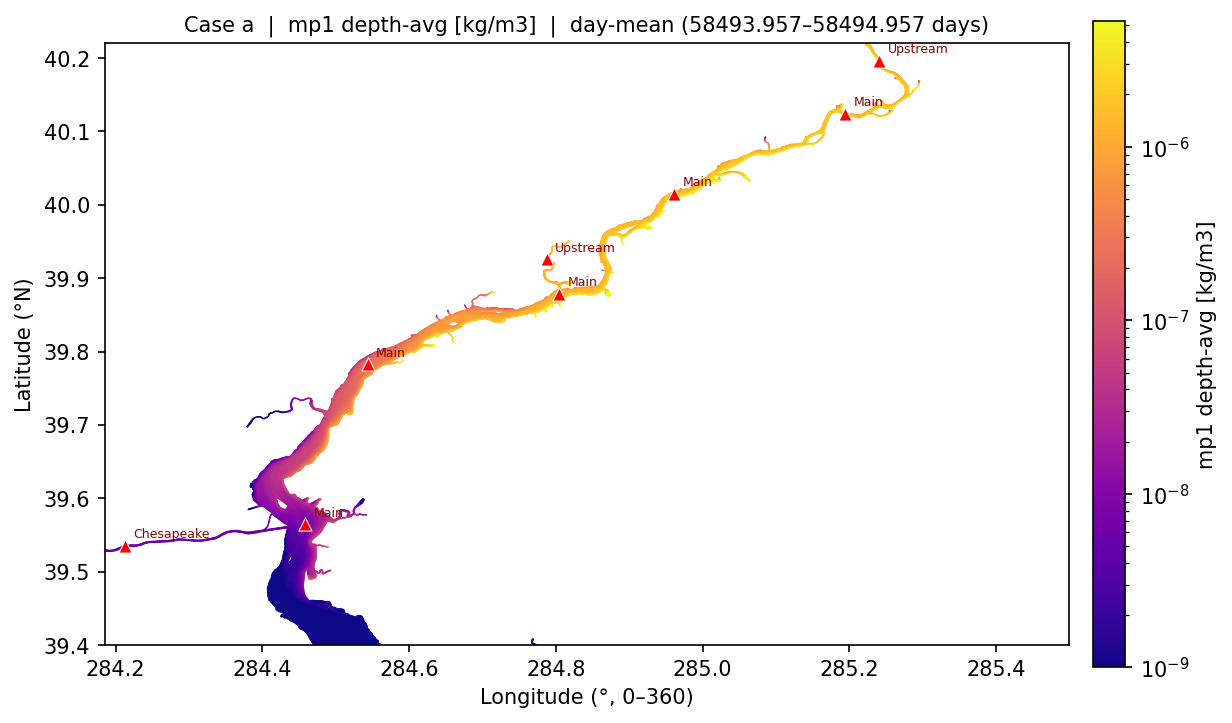
\includegraphics[width=\textwidth]{../FVCOM_MP_test_run/PYTHON/output/spatial_distribution/planview_dayavg_mp1_davg_casea.png}
  \caption{Case a — mp1 depth-averaged}
\end{subfigure}
\hfill
\begin{subfigure}[b]{0.48\textwidth}
  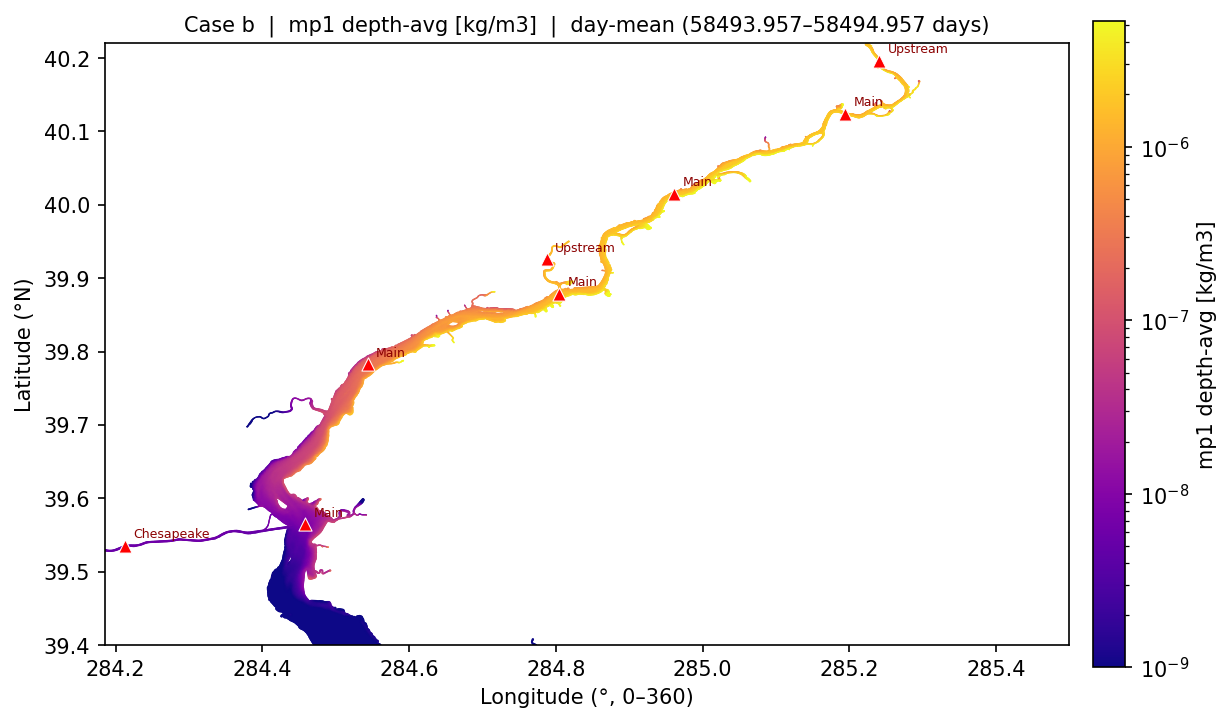
\includegraphics[width=\textwidth]{../FVCOM_MP_test_run/PYTHON/output/spatial_distribution/planview_dayavg_mp1_davg_caseb.png}
  \caption{Case b — mp1 depth-averaged}
\end{subfigure}
\caption{Day-mean depth-averaged mp1 concentration [$\mathrm{kg\,m^{-3}}$]
         over the last 24 hours of simulation.  Source locations are at the
         nine river mouths.}
\label{fig:davg_mp1}
\end{figure}

\begin{figure}[h]
\centering
\begin{subfigure}[b]{0.48\textwidth}
  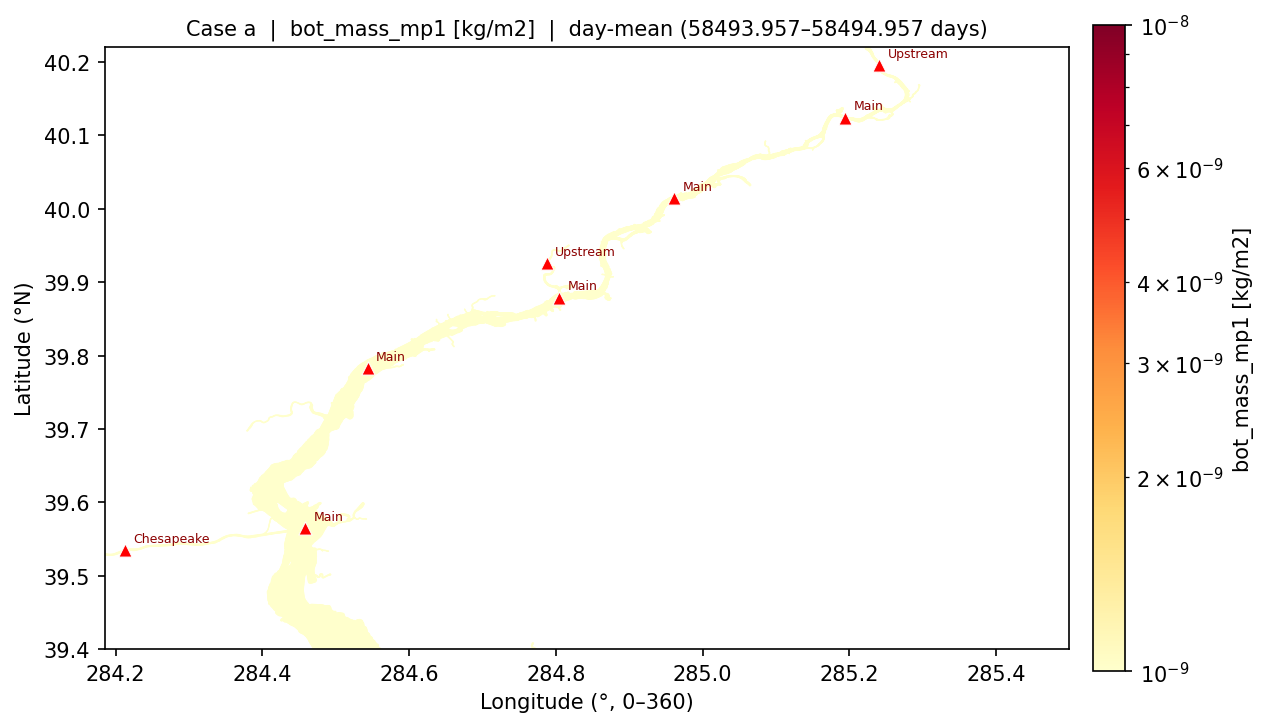
\includegraphics[width=\textwidth]{../FVCOM_MP_test_run/PYTHON/output/spatial_distribution/planview_dayavg_bot_mass_casea.png}
  \caption{Case a — bot\_mass\_mp1}
\end{subfigure}
\hfill
\begin{subfigure}[b]{0.48\textwidth}
  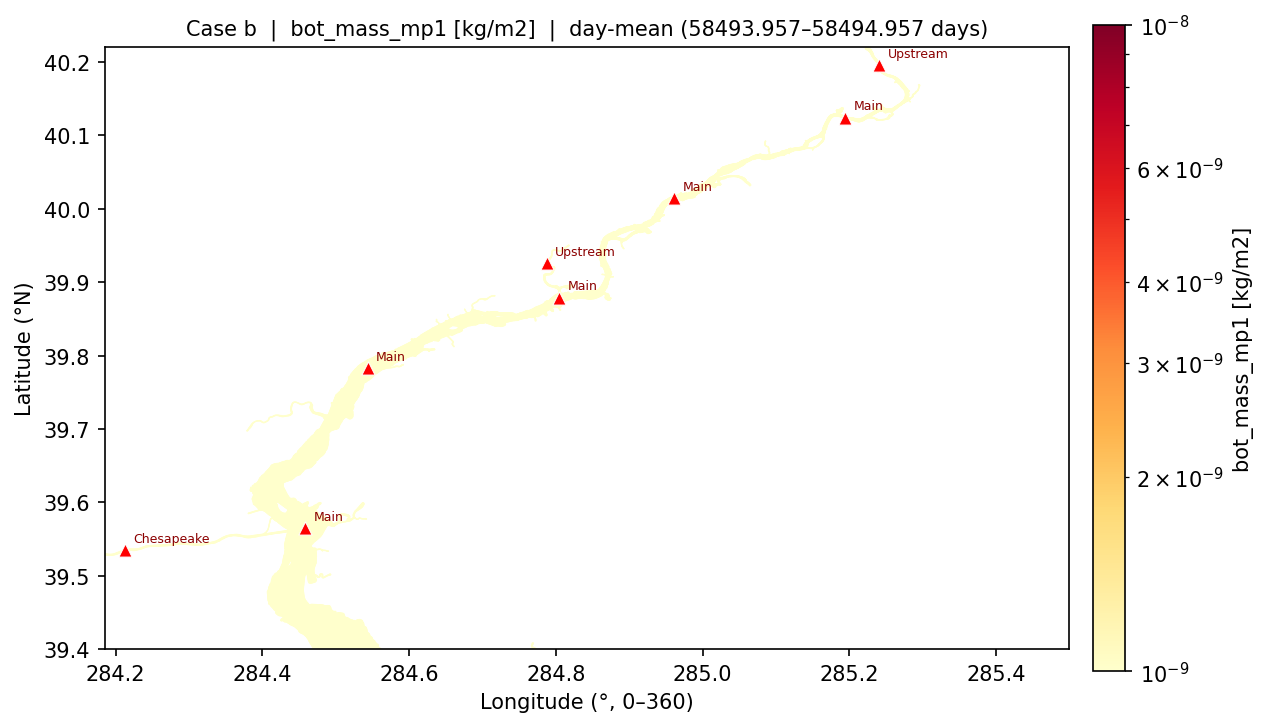
\includegraphics[width=\textwidth]{../FVCOM_MP_test_run/PYTHON/output/spatial_distribution/planview_dayavg_bot_mass_caseb.png}
  \caption{Case b — bot\_mass\_mp1}
\end{subfigure}
\caption{Day-mean bed plastic mass density [$\mathrm{kg\,m^{-2}}$]
         over the last 24 hours.}
\label{fig:bot_mass}
\end{figure}

\subsection*{Pointwise-Maximum Maps}

% ── PLACEHOLDER ──────────────────────────────────────────────────────────
\begin{figure}[h]
\centering
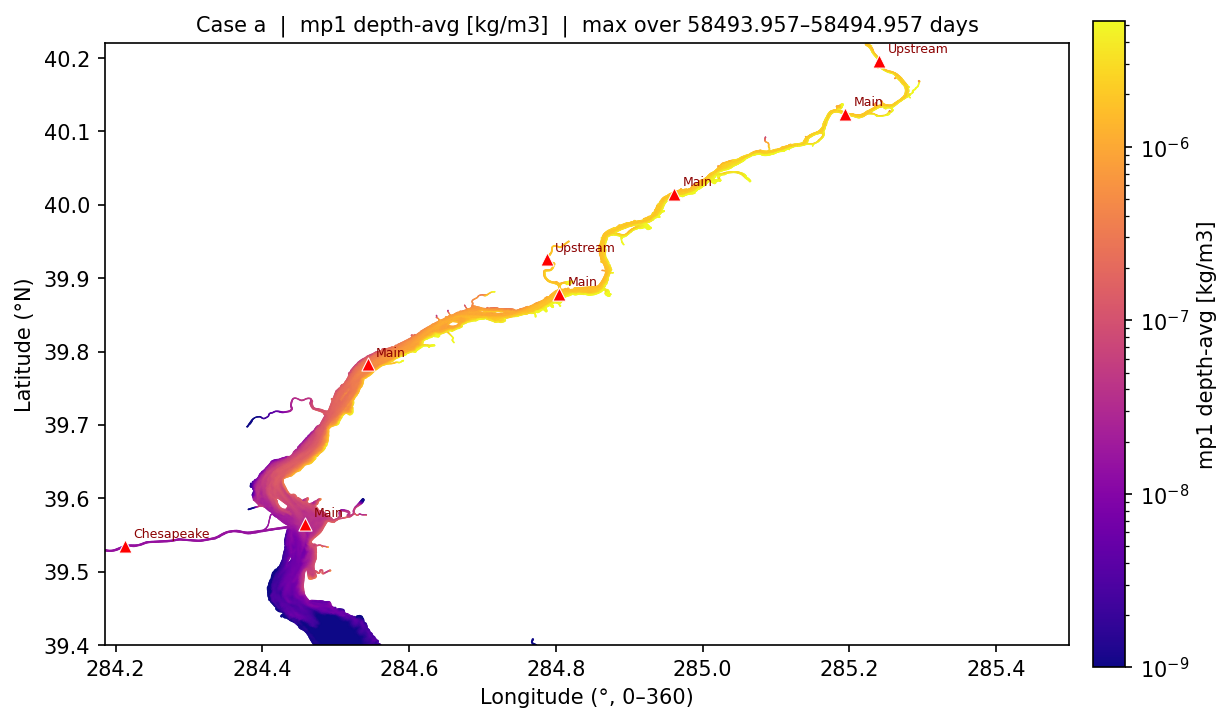
\includegraphics[width=0.6\textwidth]{../FVCOM_MP_test_run/PYTHON/output/spatial_distribution/planview_max_mp1_davg_casea.png}
\caption{Pointwise maximum depth-averaged mp1 over the last 24 hours,
         case~a.  Hotspots (if any) would indicate localised numerical
         accumulation.}
\label{fig:max_mp1}
\end{figure}

\subsection*{Cross-Case Difference Maps}

% ── PLACEHOLDER ──────────────────────────────────────────────────────────
\begin{figure}[h]
\centering
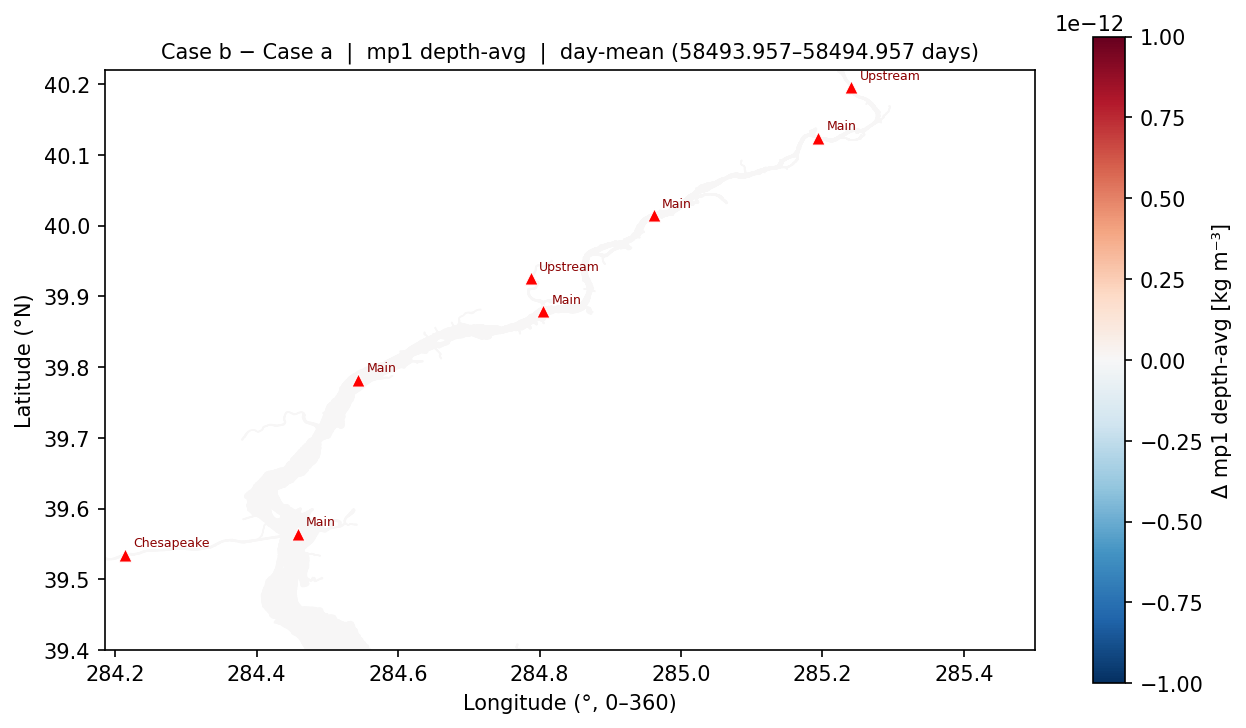
\includegraphics[width=0.6\textwidth]{../FVCOM_MP_test_run/PYTHON/output/spatial_distribution/diff_mp1_davg_caseb_minus_casea.png}
\caption{Day-mean mp1 depth-averaged difference: case~b $-$ case~a.
         Blue = less plastic in floc case; red = more.}
\label{fig:diff_mp1_ba}
\end{figure}

\subsection*{Station Time Series}

% ── PLACEHOLDER ──────────────────────────────────────────────────────────
\begin{figure}[h]
\centering
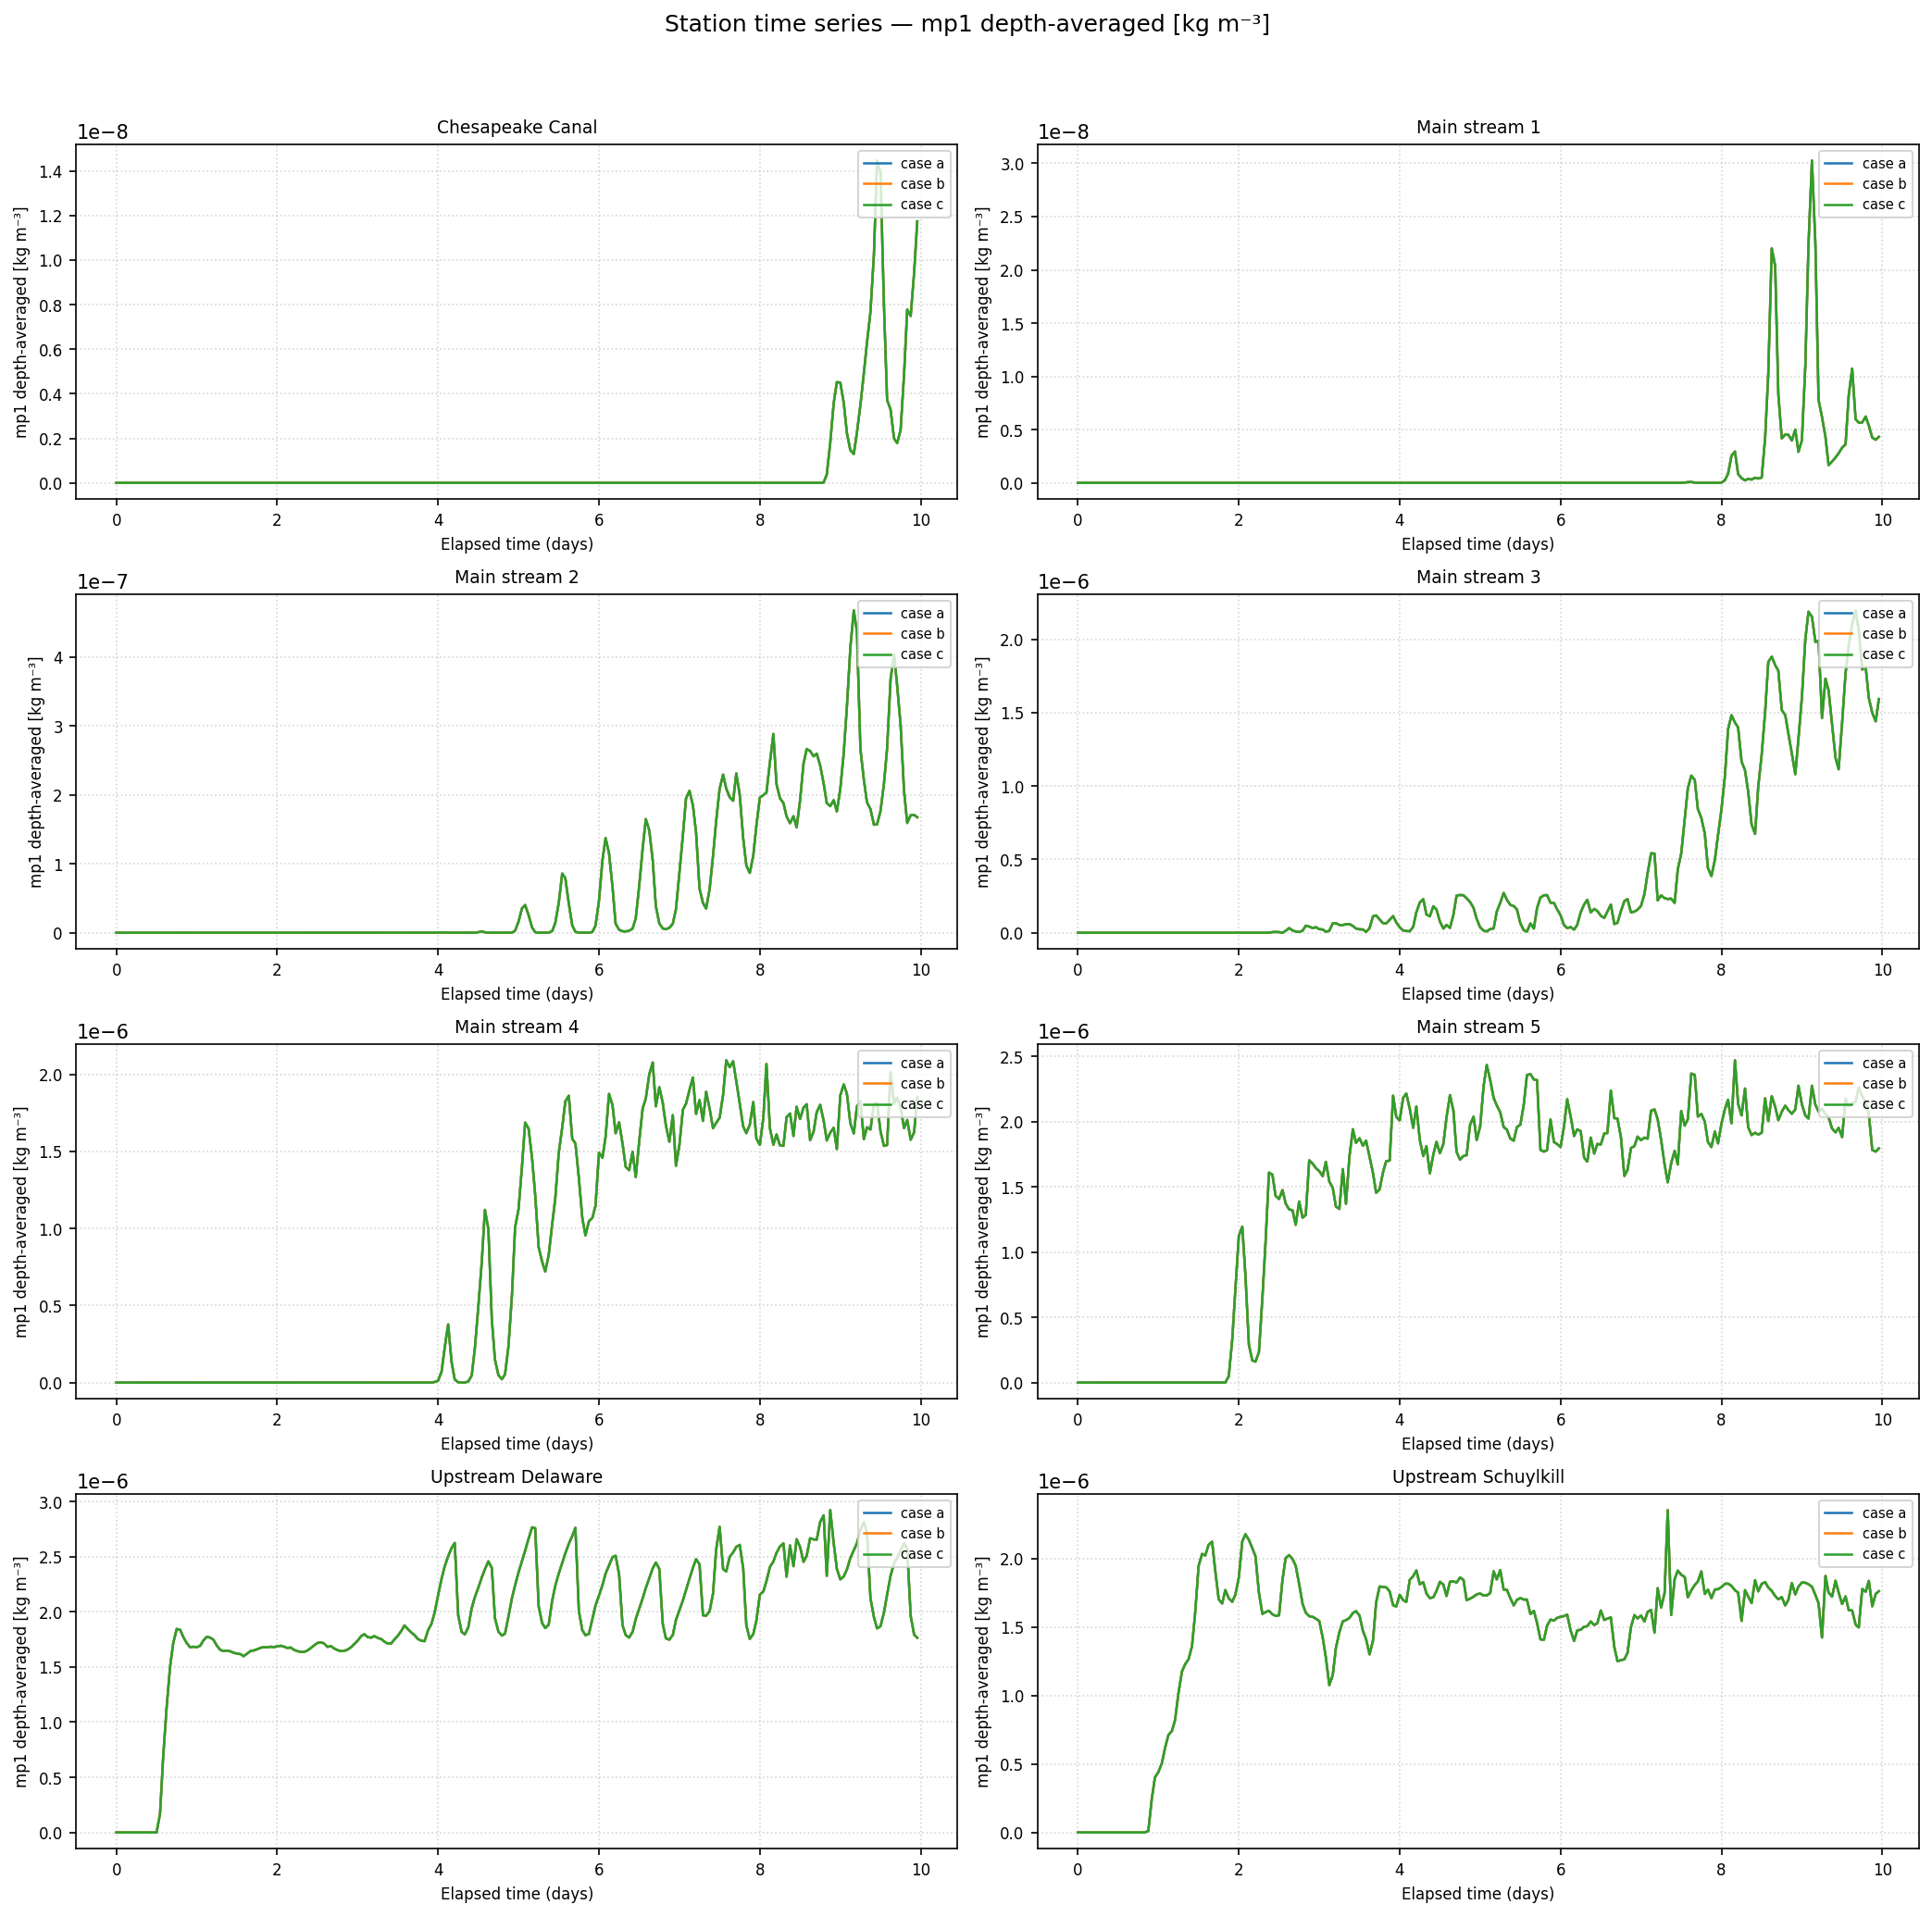
\includegraphics[width=\textwidth]{../FVCOM_MP_test_run/PYTHON/output/spatial_distribution/station_timeseries_mp1_davg.png}
\caption{Depth-averaged mp1 time series at the eight monitoring stations
         for all three cases.  Blue: case~a; orange: case~b; green:~case~c.}
\label{fig:station_mp1}
\end{figure}

\section*{Observations}

% ── TO BE FILLED IN after reviewing the figures ───────────────────────────
\textit{This section will be completed after reviewing the plots generated
by the Python analysis script.  The following items should be addressed:}

\begin{enumerate}[(1)]
  \item \textbf{Spatial extent of plastic:} does the plume extend realistically
        downstream of the river sources?  Are there any cells with
        unexpectedly high concentrations ($> 10^{-2}~\mathrm{kg\,m^{-3}}$)?
  \item \textbf{Bed accumulation pattern:} are bed deposits concentrated near
        the river mouths and along the main channel, as expected from the
        tidal forcing?
  \item \textbf{Floc-case differences (cases b/c vs.\ a):} does aggregation
        (PLAST\_FLOC=T) produce noticeably different horizontal distributions?
        Where is the sign of the difference most pronounced?
  \item \textbf{Sediment distribution (cases b/c):} is the \texttt{coarse\_sand\_1}
        field physically consistent with the bathymetry and tidal currents?
  \item \textbf{Station time series:} do the stations downstream of sources
        show coherent tidal oscillations?  Are there stations where the three
        cases diverge significantly after day~5?
  \item \textbf{Numerical anomalies:} are there isolated hotspot nodes in the
        pointwise-max maps that are not connected to any river source?  If so,
        report the node index, lon/lat, depth, and peak concentration.
\end{enumerate}

\section*{Summary and Next Steps}

% ── TO BE FILLED IN ───────────────────────────────────────────────────────
\textit{Summary to be written after observations are recorded.}

Potential next steps:
\begin{itemize}
  \item Extended 30-day runs (confirmed to be mass-conservative per Memo~04)
        to verify longer-term spatial spreading and floc-component evolution.
  \item Open-boundary hypothesis testing: instrument OBC fluxes at the
        southern bay mouth to quantify tidal export of plastic.
  \item Fix~D: multi-species flux limiting when \texttt{SOURCE\_AG\_RATE} $> 0$
        causes \texttt{conc\_a} $> 0$, which is excluded from the current
        10-day tests but required for full-physics runs.
\end{itemize}

\end{document}
